\newpage
%début et titre de la sous-section
\subsection{The protective case}

\begin{figure}[!h]
    \centering
    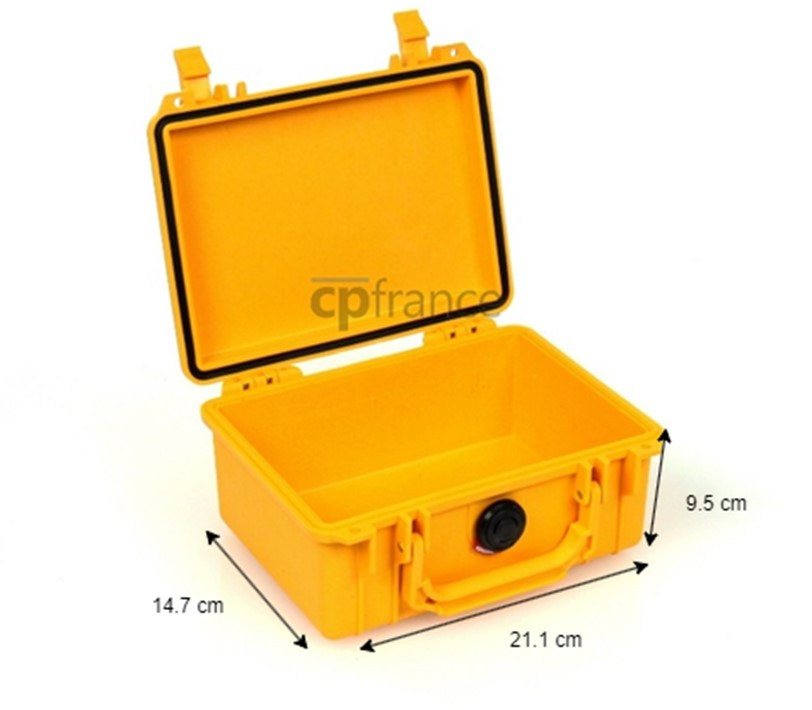
\includegraphics[width=0.8\textwidth]{\currfiledir/figures/case.jpg}
    \caption{Valise Peli™ 1150}
    \cite{case}
\end{figure}

The protective case has a role of protecting the whole system from the outside elements. The housing of the recording system needs to withstand extreme weather conditions, such as high temperatures (which can reach up to 35°C in Gabon), high humidity (up to 90\%), rain, and potential animal interference. To reduce wind-induced vibrations, a small plastic housing with a rubber seal was chosen (Protector 1150, Peli) to hold the camera, control unit, and GPS receiver.